\documentclass{report}

%%%%%%%%%%%%%%%%%%%%%%%%%%%%%%%%
% PACKAGE IMPORTS
%%%%%%%%%%%%%%%%%%%%%%%%%%%%%%%%%


\usepackage[tmargin=2cm,rmargin=1in,lmargin=1in,margin=0.85in,bmargin=2cm,footskip=.2in]{geometry}
\usepackage{amsmath,amsfonts,amsthm,amssymb,mathtools}
\usepackage[varbb]{newpxmath}
\usepackage{xfrac}
\usepackage[makeroom]{cancel}
\usepackage{mathtools}
\usepackage{bookmark}
\usepackage{enumitem}
\usepackage{hyperref,theoremref}
\hypersetup{
	pdftitle={Assignment},
	colorlinks=true, linkcolor=doc!90,
	bookmarksnumbered=true,
	bookmarksopen=true
}
\usepackage[most,many,breakable]{tcolorbox}
\usepackage{xcolor}
\usepackage{varwidth}
\usepackage{varwidth}
\usepackage{etoolbox}
%\usepackage{authblk}
\usepackage{nameref}
\usepackage{multicol,array}
\usepackage{tikz-cd}
\usepackage{tikz-3dplot}
\usepackage[ruled,vlined,linesnumbered]{algorithm2e}
\usepackage{comment} % enables the use of multi-line comments (\ifx \fi) 
\usepackage{import}
\usepackage{xifthen}
\usepackage{pdfpages}
\usepackage{transparent}
\usepackage{graphicx} % <-- Added package to handle graphics
\usepackage{xcolor}
\usepackage{pgfplots}
\usepackage{minted}
\definecolor{pastelFDF7C3}{HTML}{FDF7C3}
\pgfplotsset{compat=newest}
\usepgfplotslibrary{colormaps}


\newcommand\mycommfont[1]{\footnotesize\ttfamily\textcolor{blue}{#1}}
\SetCommentSty{mycommfont}
\newcommand{\incfig}[1]{%
    \def\svgwidth{\columnwidth}
    \import{./figures/}{#1.pdf_tex}
}

\usepackage{tikzsymbols}
\renewcommand\qedsymbol{$\Laughey$}


%\usepackage{import}
%\usepackage{xifthen}
%\usepackage{pdfpages}
%\usepackage{transparent}


%%%%%%%%%%%%%%%%%%%%%%%%%%%%%%
% SELF MADE COLORS
%%%%%%%%%%%%%%%%%%%%%%%%%%%%%%



\definecolor{myg}{RGB}{56, 140, 70}
\definecolor{myb}{RGB}{45, 111, 177}
\definecolor{myr}{RGB}{199, 68, 64}
\definecolor{mytheorembg}{HTML}{F2F2F9}
\definecolor{mytheoremfr}{HTML}{00007B}
\definecolor{mylenmabg}{HTML}{FFFAF8}
\definecolor{mylenmafr}{HTML}{983b0f}
\definecolor{mypropbg}{HTML}{f2fbfc}
\definecolor{mypropfr}{HTML}{191971}
\definecolor{myexamplebg}{HTML}{F2FBF8}
\definecolor{myexamplefr}{HTML}{88D6D1}
\definecolor{myexampleti}{HTML}{2A7F7F}
\definecolor{mydefinitbg}{HTML}{E5E5FF}
\definecolor{mydefinitfr}{HTML}{3F3FA3}
\definecolor{notesgreen}{RGB}{0,162,0}
\definecolor{myp}{RGB}{197, 92, 212}
\definecolor{mygr}{HTML}{2C3338}
\definecolor{myred}{RGB}{127,0,0}
\definecolor{myyellow}{RGB}{169,121,69}
\definecolor{myexercisebg}{HTML}{F2FBF8}
\definecolor{myexercisefg}{HTML}{88D6D1}


%%%%%%%%%%%%%%%%%%%%%%%%%%%%
% TCOLORBOX SETUPS
%%%%%%%%%%%%%%%%%%%%%%%%%%%%

\setlength{\parindent}{1cm}
%================================
% THEOREM BOX
%================================

\tcbuselibrary{theorems,skins,hooks}
\newtcbtheorem[number within=section]{Theorem}{Theorem}
{%
	enhanced,
	breakable,
	colback = mytheorembg,
	frame hidden,
	boxrule = 0sp,
	borderline west = {2pt}{0pt}{mytheoremfr},
	sharp corners,
	detach title,
	before upper = \tcbtitle\par\smallskip,
	coltitle = mytheoremfr,
	fonttitle = \bfseries\sffamily,
	description font = \mdseries,
	separator sign none,
	segmentation style={solid, mytheoremfr},
}
{th}

\tcbuselibrary{theorems,skins,hooks}
\newtcbtheorem[number within=chapter]{theorem}{Theorem}
{%
	enhanced,
	breakable,
	colback = mytheorembg,
	frame hidden,
	boxrule = 0sp,
	borderline west = {2pt}{0pt}{mytheoremfr},
	sharp corners,
	detach title,
	before upper = \tcbtitle\par\smallskip,
	coltitle = mytheoremfr,
	fonttitle = \bfseries\sffamily,
	description font = \mdseries,
	separator sign none,
	segmentation style={solid, mytheoremfr},
}
{th}


\tcbuselibrary{theorems,skins,hooks}
\newtcolorbox{Theoremcon}
{%
	enhanced
	,breakable
	,colback = mytheorembg
	,frame hidden
	,boxrule = 0sp
	,borderline west = {2pt}{0pt}{mytheoremfr}
	,sharp corners
	,description font = \mdseries
	,separator sign none
}

%================================
% Corollery
%================================
\tcbuselibrary{theorems,skins,hooks}
\newtcbtheorem[number within=section]{Corollary}{Corollary}
{%
	enhanced
	,breakable
	,colback = myp!10
	,frame hidden
	,boxrule = 0sp
	,borderline west = {2pt}{0pt}{myp!85!black}
	,sharp corners
	,detach title
	,before upper = \tcbtitle\par\smallskip
	,coltitle = myp!85!black
	,fonttitle = \bfseries\sffamily
	,description font = \mdseries
	,separator sign none
	,segmentation style={solid, myp!85!black}
}
{th}
\tcbuselibrary{theorems,skins,hooks}
\newtcbtheorem[number within=chapter]{corollary}{Corollary}
{%
	enhanced
	,breakable
	,colback = myp!10
	,frame hidden
	,boxrule = 0sp
	,borderline west = {2pt}{0pt}{myp!85!black}
	,sharp corners
	,detach title
	,before upper = \tcbtitle\par\smallskip
	,coltitle = myp!85!black
	,fonttitle = \bfseries\sffamily
	,description font = \mdseries
	,separator sign none
	,segmentation style={solid, myp!85!black}
}
{th}


%================================
% LENMA
%================================

\tcbuselibrary{theorems,skins,hooks}
\newtcbtheorem[number within=section]{Lenma}{Lenma}
{%
	enhanced,
	breakable,
	colback = mylenmabg,
	frame hidden,
	boxrule = 0sp,
	borderline west = {2pt}{0pt}{mylenmafr},
	sharp corners,
	detach title,
	before upper = \tcbtitle\par\smallskip,
	coltitle = mylenmafr,
	fonttitle = \bfseries\sffamily,
	description font = \mdseries,
	separator sign none,
	segmentation style={solid, mylenmafr},
}
{th}

\tcbuselibrary{theorems,skins,hooks}
\newtcbtheorem[number within=chapter]{lenma}{Lenma}
{%
	enhanced,
	breakable,
	colback = mylenmabg,
	frame hidden,
	boxrule = 0sp,
	borderline west = {2pt}{0pt}{mylenmafr},
	sharp corners,
	detach title,
	before upper = \tcbtitle\par\smallskip,
	coltitle = mylenmafr,
	fonttitle = \bfseries\sffamily,
	description font = \mdseries,
	separator sign none,
	segmentation style={solid, mylenmafr},
}
{th}


%================================
% PROPOSITION
%================================

\tcbuselibrary{theorems,skins,hooks}
\newtcbtheorem[number within=section]{Prop}{Proposition}
{%
	enhanced,
	breakable,
	colback = mypropbg,
	frame hidden,
	boxrule = 0sp,
	borderline west = {2pt}{0pt}{mypropfr},
	sharp corners,
	detach title,
	before upper = \tcbtitle\par\smallskip,
	coltitle = mypropfr,
	fonttitle = \bfseries\sffamily,
	description font = \mdseries,
	separator sign none,
	segmentation style={solid, mypropfr},
}
{th}

\tcbuselibrary{theorems,skins,hooks}
\newtcbtheorem[number within=chapter]{prop}{Proposition}
{%
	enhanced,
	breakable,
	colback = mypropbg,
	frame hidden,
	boxrule = 0sp,
	borderline west = {2pt}{0pt}{mypropfr},
	sharp corners,
	detach title,
	before upper = \tcbtitle\par\smallskip,
	coltitle = mypropfr,
	fonttitle = \bfseries\sffamily,
	description font = \mdseries,
	separator sign none,
	segmentation style={solid, mypropfr},
}
{th}


%================================
% CLAIM
%================================

\tcbuselibrary{theorems,skins,hooks}
\newtcbtheorem[number within=section]{claim}{Claim}
{%
	enhanced
	,breakable
	,colback = myg!10
	,frame hidden
	,boxrule = 0sp
	,borderline west = {2pt}{0pt}{myg}
	,sharp corners
	,detach title
	,before upper = \tcbtitle\par\smallskip
	,coltitle = myg!85!black
	,fonttitle = \bfseries\sffamily
	,description font = \mdseries
	,separator sign none
	,segmentation style={solid, myg!85!black}
}
{th}



%================================
% Exercise
%================================

\tcbuselibrary{theorems,skins,hooks}
\newtcbtheorem[number within=section]{Exercise}{Exercise}
{%
	enhanced,
	breakable,
	colback = myexercisebg,
	frame hidden,
	boxrule = 0sp,
	borderline west = {2pt}{0pt}{myexercisefg},
	sharp corners,
	detach title,
	before upper = \tcbtitle\par\smallskip,
	coltitle = myexercisefg,
	fonttitle = \bfseries\sffamily,
	description font = \mdseries,
	separator sign none,
	segmentation style={solid, myexercisefg},
}
{th}

\tcbuselibrary{theorems,skins,hooks}
\newtcbtheorem[number within=chapter]{exercise}{Exercise}
{%
	enhanced,
	breakable,
	colback = myexercisebg,
	frame hidden,
	boxrule = 0sp,
	borderline west = {2pt}{0pt}{myexercisefg},
	sharp corners,
	detach title,
	before upper = \tcbtitle\par\smallskip,
	coltitle = myexercisefg,
	fonttitle = \bfseries\sffamily,
	description font = \mdseries,
	separator sign none,
	segmentation style={solid, myexercisefg},
}
{th}

%================================
% EXAMPLE BOX (Lighter Pastel Purple)
%================================

\definecolor{pastelExampleBg}{HTML}{70AF85} % Base pastel color
\definecolor{greenPast}{HTML}{86C8BC} % Base pastel color
\colorlet{myexamplebg}{pastelExampleBg!25!white} % Mix with white for a pastel color
\colorlet{myexamplefr}{pastelExampleBg!85!white} % Use the same mix for the frame
\colorlet{myexampleti}{greenPast!40!black} % Mix A1EEBD with black for a darker green

\newtcbtheorem[number within=section]{Example}{Example}
{%
	colback = myexamplebg
	,breakable
	,colframe = myexamplefr
	,coltitle = myexampleti
	,boxrule = 1pt
	,sharp corners
	,detach title
	,before upper=\tcbtitle\par\smallskip
	,fonttitle = \bfseries
	,description font = \mdseries
	,separator sign none
	,description delimiters parenthesis
}
{ex}

\newtcbtheorem[number within=chapter]{example}{Example}
{%
	colback = myexamplebg
	,breakable
	,colframe = myexamplefr
	,coltitle = myexampleti
	,boxrule = 1pt
	,sharp corners
	,detach title
	,before upper=\tcbtitle\par\smallskip
	,fonttitle = \bfseries
	,description font = \mdseries
	,separator sign none
	,description delimiters parenthesis
}
{ex}

%================================
% EXAMPLE BOX (Rose)
%================================

% Define the custom example box with rose image in the top-right corner
\newtcolorbox[auto counter, number within=section]{ExampleWithRose}[2][]{%
    colback=myexamplebg,  % Use the pastel version of BFF6C3 for the background
    colframe=myexamplefr, % Use the pastel version of BFF6C3 for the frame
    coltitle=myexampleti, % Use black for the title color
    fonttitle=\bfseries,
    title={Example~\thetcbcounter: #2},
    sharp corners,
    enhanced,
    overlay={
        \node[anchor=south east] at (frame.south east) {
\includegraphics[width=1.5cm]{flow.png}};
    },
    #1
}

%================================
% DEFINITION BOX
%================================

\makeatletter
\definecolor{customblue}{RGB}{198, 220, 228} % Custom blue color
\definecolor{darkblue}{RGB}{90, 120, 140} % Darker blue for text

\newtcbtheorem[number within=section]{Definition}{Definition}{enhanced,
	before skip=2mm,after skip=2mm, colback=customblue!20,colframe=customblue!80,boxrule=0.5mm,
	attach boxed title to top left={xshift=1cm,yshift*=1mm-\tcboxedtitleheight}, varwidth boxed title*=-3cm,
	boxed title style={frame code={
					\path[fill=customblue]  % Custom blue fill
					([yshift=-1mm,xshift=-1mm]frame.north west)
					arc[start angle=0,end angle=180,radius=1mm]
					([yshift=-1mm,xshift=1mm]frame.north east)
					arc[start angle=180,end angle=0,radius=1mm];
					\path[left color=customblue,right color=customblue,
						middle color=customblue!90]  % Light custom blue gradient
					([xshift=-2mm]frame.north west) -- ([xshift=2mm]frame.north east)
					[rounded corners=1mm]-- ([xshift=1mm,yshift=-1mm]frame.north east)
					-- (frame.south east) -- (frame.south west)
					-- ([xshift=-1mm,yshift=-1mm]frame.north west)
					[sharp corners]-- cycle;
				},interior engine=empty,
		},
	fonttitle=\bfseries\color{darkblue}, % Darker blue for the title text
	coltitle=darkblue, % Darker blue for the box title
	colbacktitle=customblue!80, % Background for the title
	title={#2},#1}{def}

\newtcbtheorem[number within=chapter]{definition}{Definition}{enhanced,
	before skip=2mm,after skip=2mm, colback=customblue!20,colframe=customblue!80,boxrule=0.5mm,
	attach boxed title to top left={xshift=1cm,yshift*=1mm-\tcboxedtitleheight}, varwidth boxed title*=-3cm,
	boxed title style={frame code={
					\path[fill=customblue]  % Custom blue fill
					([yshift=-1mm,xshift=-1mm]frame.north west)
					arc[start angle=0,end angle=180,radius=1mm]
					([yshift=-1mm,xshift=1mm]frame.north east)
					arc[start angle=180,end angle=0,radius=1mm];
					\path[left color=customblue,right color=customblue,
						middle color=customblue!90]  % Light custom blue gradient
					([xshift=-2mm]frame.north west) -- ([xshift=2mm]frame.north east)
					[rounded corners=1mm]-- ([xshift=1mm,yshift=-1mm]frame.north east)
					-- (frame.south east) -- (frame.south west)
					-- ([xshift=-1mm,yshift=-1mm]frame.north west)
					[sharp corners]-- cycle;
				},interior engine=empty,
		},
	fonttitle=\bfseries\color{darkblue}, % Darker blue for the title text
	coltitle=darkblue, % Darker blue for the box title
	colbacktitle=customblue!80, % Background for the title
	title={#2},#1}{def}
\makeatother

%================================
% DEFINITION BOX WITH IMAGE IN BOTTOM-RIGHT
%================================

%================================
% DEFINITION BOX WITH IMAGE IN BOTTOM-RIGHT
%================================

\makeatletter
\definecolor{customblue}{RGB}{198, 234, 245} % Custom blue color
\definecolor{darkblue}{RGB}{90, 120, 140} % Darker blue for text

\newtcbtheorem[number within=section]{DefinitionWithImage}{Definition}{enhanced,
	before skip=2mm,
	after skip=2mm, 
	colback=customblue!40, % Use custom blue with 20% intensity for background
	colframe=customblue!80!black, % Use custom blue with some black for the frame
	boxrule=0.5mm,
	attach boxed title to top left={xshift=1cm,yshift*=1mm-\tcboxedtitleheight}, 
	varwidth boxed title*=-3cm,
	boxed title style={frame code={
					\path[fill=customblue]  % Custom blue fill
					([yshift=-1mm,xshift=-1mm]frame.north west)
					arc[start angle=0,end angle=180,radius=1mm]
					([yshift=-1mm,xshift=1mm]frame.north east)
					arc[start angle=180,end angle=0,radius=1mm];
					\path[left color=customblue,right color=customblue,
						middle color=customblue!90]  % Light custom blue gradient
					([xshift=-2mm]frame.north west) -- ([xshift=2mm]frame.north east)
					[rounded corners=1mm]-- ([xshift=1mm,yshift=-1mm]frame.north east)
					-- (frame.south east) -- (frame.south west)
					-- ([xshift=-1mm,yshift=-1mm]frame.north west)
					[sharp corners]-- cycle;
				},interior engine=empty,
		},
	fonttitle=\bfseries\color{darkblue}, % Darker blue for the title text
	coltitle=darkblue, % Darker blue for the box title
	colbacktitle=customblue!80, % Background for the title
	title={#2},
	overlay unbroken and last={
		\node[anchor=south east,xshift=-2mm,yshift=2mm] at (frame.south east) {
\includegraphics[width=1 cm]{slime.png}};
	} % Adjust the path and size to your needs
}{def}
\makeatother

%================================
% Solution BOX (Pastel Light Blue)
%================================

\makeatletter
\definecolor{pastelpink}{HTML}{FFE3ED} % Define pastel pink using the hex code #FFE3ED

\newtcbtheorem{question}{Question}{enhanced,
	breakable,
	colback=pastelpink!60, % Use pastel pink for the background with 60% intensity
	colframe=pastelpink!90!black, % Use pastel pink with a bit of black for the frame
	attach boxed title to top left={yshift*=-\tcboxedtitleheight},
	fonttitle=\bfseries,
	title={#2},
	boxed title size=title,
	boxed title style={%
			sharp corners,
			rounded corners=northwest,
			colback=tcbcolframe,
			boxrule=0pt,
		},
	underlay boxed title={%
			\path[fill=tcbcolframe] (title.south west)--(title.south east)
			to[out=0, in=180] ([xshift=5mm]title.east)--
			(title.center-|frame.east)
			[rounded corners=\kvtcb@arc] |-
			(frame.north) -| cycle;
		},
	#1
}{def}
\makeatother


% SOLUTION BOX
%================================

\makeatletter
\newtcolorbox{solution}{enhanced,
	breakable,
	colback=white,
	colframe=myg!80!black,
	attach boxed title to top left={yshift*=-\tcboxedtitleheight},
	title=Solution,
	boxed title size=title,
	boxed title style={%
			sharp corners,
			rounded corners=northwest,
			colback=tcbcolframe,
			boxrule=0pt,
		},
	underlay boxed title={%
			\path[fill=tcbcolframe] (title.south west)--(title.south east)
			to[out=0, in=180] ([xshift=5mm]title.east)--
			(title.center-|frame.east)
			[rounded corners=\kvtcb@arc] |-
			(frame.north) -| cycle;
		},
}
\makeatother

%================================
% Question BOX
%================================

\makeatletter
\newtcbtheorem{qstion}{Question}{enhanced,
	breakable,
	colback=white,
	colframe=mygr,
	attach boxed title to top left={yshift*=-\tcboxedtitleheight},
	fonttitle=\bfseries,
	title={#2},
	boxed title size=title,
	boxed title style={%
			sharp corners,
			rounded corners=northwest,
			colback=tcbcolframe,
			boxrule=0pt,
		},
	underlay boxed title={%
			\path[fill=tcbcolframe] (title.south west)--(title.south east)
			to[out=0, in=180] ([xshift=5mm]title.east)--
			(title.center-|frame.east)
			[rounded corners=\kvtcb@arc] |-
			(frame.north) -| cycle;
		},
	#1
}{def}
\makeatother

\newtcbtheorem[number within=chapter]{wconc}{Wrong Concept}{
	breakable,
	enhanced,
	colback=white,
	colframe=myr,
	arc=0pt,
	outer arc=0pt,
	fonttitle=\bfseries\sffamily\large,
	colbacktitle=myr,
	attach boxed title to top left={},
	boxed title style={
			enhanced,
			skin=enhancedfirst jigsaw,
			arc=3pt,
			bottom=0pt,
			interior style={fill=myr}
		},
	#1
}{def}



%================================
% NOTE BOX (Pastel Pink)
%================================

\usetikzlibrary{arrows,calc,shadows.blur}
\tcbuselibrary{skins}
\definecolor{pastelpink}{HTML}{FFE3ED} % Define pastel pink using the hex code #FFE3ED

\newtcolorbox{note}[1][]{%
    enhanced jigsaw,
    colback=pastelpink, % Use pastel pink for the background
    colframe=pastelpink, % Use pastel pink for the frame
    size=small,
    boxrule=1pt,
    title=\textbf{Note:-},
    halign title=flush center,
    coltitle=black,
    breakable,
    drop shadow=black!50!white,
    attach boxed title to top left={xshift=1cm,yshift=-\tcboxedtitleheight/2,yshifttext=-\tcboxedtitleheight/2},
    minipage boxed title=1.5cm,
    boxed title style={%
            colback=white,
            size=fbox,
            boxrule=1pt,
            boxsep=2pt,
            underlay={%
                    \coordinate (dotA) at ($(interior.west) + (-0.5pt,0)$);
                    \coordinate (dotB) at ($(interior.east) + (0.5pt,0)$);
                    \begin{scope}
                        \clip (interior.north west) rectangle ([xshift=3ex]interior.east);
                        \filldraw [white, blur shadow={shadow opacity=60, shadow yshift=-.75ex}, rounded corners=2pt] (interior.north west) rectangle (interior.south east);
                    \end{scope}
                    \begin{scope}[pastelpink]
                        \fill (dotA) circle (2pt);
                        \fill (dotB) circle (2pt);
                    \end{scope}
                },
        },
    #1,
}

%================================
% NOTE BOX (Pastel Pink with Image in Bottom-Left)
%================================
\newtcolorbox{noteWithImage}[1][]{%
    enhanced jigsaw,
    colback=pastelFDF7C3!70!white, % Mix pastelFDF7C3 with white to lighten the color
    colframe=pastelFDF7C3!80!white, % Mix pastelFDF7C3 with white for the frame
    size=small,
    boxrule=1pt,
    title=\textbf{Note:-},
    halign title=flush center,
    coltitle=black,
    breakable,
    drop shadow=black!50!white,
    attach boxed title to top left={xshift=1cm,yshift=-\tcboxedtitleheight/2,yshifttext=-\tcboxedtitleheight/2},
    minipage boxed title=1.5cm,
    boxed title style={%
            colback=white,
            size=fbox,
            boxrule=1pt,
            boxsep=2pt,
            underlay={%
                    \coordinate (dotA) at ($(interior.west) + (-0.5pt,0)$);
                    \coordinate (dotB) at ($(interior.east) + (0.5pt,0)$);
                    \begin{scope}
                        \clip (interior.north west) rectangle ([xshift=3ex]interior.east);
                        \filldraw [white, blur shadow={shadow opacity=60, shadow yshift=-.75ex}, rounded corners=2pt] (interior.north west) rectangle (interior.south east);
                    \end{scope}
                    \begin{scope}[pastelFDF7C3!80!white]
                        \fill (dotA) circle (2pt);
                        \fill (dotB) circle (2pt);
                    \end{scope}
                },
        },
    overlay unbroken and last={
        \node[anchor=south east,xshift=-2mm,yshift=1mm] at (frame.south east) {
\includegraphics[width=1cm]{lot.png}};
    }, % Replace 'rose.png' with the path to your image
    #1,
}


%%%%%%%%%%%%%%%%%%%%%%%%%%%%%%
% SELF MADE COMMANDS
%%%%%%%%%%%%%%%%%%%%%%%%%%%%%%


\newcommand{\thm}[2]{\begin{Theorem}{#1}{}#2\end{Theorem}}
\newcommand{\cor}[2]{\begin{Corollary}{#1}{}#2\end{Corollary}}
\newcommand{\mlenma}[2]{\begin{Lenma}{#1}{}#2\end{Lenma}}
\newcommand{\mprop}[2]{\begin{Prop}{#1}{}#2\end{Prop}}
\newcommand{\clm}[3]{\begin{claim}{#1}{#2}#3\end{claim}}
\newcommand{\wc}[2]{\begin{wconc}{#1}{}\setlength{\parindent}{1cm}#2\end{wconc}}
\newcommand{\thmcon}[1]{\begin{Theoremcon}{#1}\end{Theoremcon}}
\newcommand{\exer}[2]{\begin{Exercise}{#1}{}#2\end{Exercise}}
\newcommand{\ex}[2]{\begin{Example}{#1}{}#2\end{Example}}
\newcommand{\dfn}[2]{\begin{Definition}[colbacktitle=red!75!black]{#1}{}#2\end{Definition}}
\newcommand{\dfnc}[2]{\begin{definition}[colbacktitle=red!75!black]{#1}{}#2\end{definition}}
\newcommand{\qs}[2]{\begin{question}{#1}{}#2\end{question}}
\newcommand{\pf}[2]{\begin{myproof}[#1]#2\end{myproof}}
\newcommand{\nt}[1]{\begin{note}#1\end{note}}
\newcommand{\insertpng}[2][1]{\begin{center} \includegraphics[scale=#1]{#2} \end{center}} % <-- New command for PNG insertion

\newcommand{\defrose}[2]{%
    \begin{DefinitionWithImage}{#1}%
        #2%
    \end{DefinitionWithImage}%
}

\newcommand{\exrose}[2]{%
    \begin{ExampleWithRose}{#1}%
        #2%
    \end{ExampleWithRose}%
}

\newcommand{\ntimg}[2][]{%
    \begin{noteWithImage}[#1]%
        #2%
    \end{noteWithImage}%
}

\newcommand*\circled[1]{\tikz[baseline=(char.base)]{
		\node[shape=circle,draw,inner sep=1pt] (char) {#1};}}
\newcommand\getcurrentref[1]{%
	\ifnumequal{\value{#1}}{0}
	{??}
	{\the\value{#1}}%
}
\newcommand{\getCurrentSectionNumber}{\getcurrentref{section}}
\newenvironment{myproof}[1][\proofname]{%
	\proof[\bfseries #1: ]%
}{\endproof}

\newcommand{\mclm}[2]{\begin{myclaim}[#1]#2\end{myclaim}}
\newenvironment{myclaim}[1][\claimname]{\proof[\bfseries #1: ]}{}

\newcounter{mylabelcounter}

\makeatletter
\newcommand{\setword}[2]{%
	\phantomsection
	#1\def\@currentlabel{\unexpanded{#1}}\label{#2}%
}
\makeatother




\tikzset{
	symbol/.style={
			draw=none,
			every to/.append style={
					edge node={node [sloped, allow upside down, auto=false]{$#1$}}}
		}
}


% deliminators
\DeclarePairedDelimiter{\abs}{\lvert}{\rvert}
\DeclarePairedDelimiter{\norm}{\lVert}{\rVert}

\DeclarePairedDelimiter{\ceil}{\lceil}{\rceil}
\DeclarePairedDelimiter{\floor}{\lfloor}{\rfloor}
\DeclarePairedDelimiter{\round}{\lfloor}{\rceil}

\newsavebox\diffdbox
\newcommand{\slantedromand}{{\mathpalette\makesl{d}}}
\newcommand{\makesl}[2]{%
\begingroup
\sbox{\diffdbox}{$\mathsurround=0pt#1\mathrm{#2}$}%
\pdfsave
\pdfsetmatrix{1 0 0.2 1}%
\rlap{\usebox{\diffdbox}}%
\pdfrestore
\hskip\wd\diffdbox
\endgroup
}
\newcommand{\dd}[1][]{\ensuremath{\mathop{}\!\ifstrempty{#1}{%
\slantedromand\@ifnextchar^{\hspace{0.2ex}}{\hspace{0.1ex}}}%
{\slantedromand\hspace{0.2ex}^{#1}}}}
\ProvideDocumentCommand\dv{o m g}{%
  \ensuremath{%
    \IfValueTF{#3}{%
      \IfNoValueTF{#1}{%
        \frac{\dd #2}{\dd #3}%
      }{%
        \frac{\dd^{#1} #2}{\dd #3^{#1}}%
      }%
    }{%
      \IfNoValueTF{#1}{%
        \frac{\dd}{\dd #2}%
      }{%
        \frac{\dd^{#1}}{\dd #2^{#1}}%
      }%
    }%
  }%
}
\providecommand*{\pdv}[3][]{\frac{\partial^{#1}#2}{\partial#3^{#1}}}
%  - others
\DeclareMathOperator{\Lap}{\mathcal{L}}
\DeclareMathOperator{\Var}{Var} % varience
\DeclareMathOperator{\Cov}{Cov} % covarience
\DeclareMathOperator{\E}{E} % expected

% Since the amsthm package isn't loaded

% I prefer the slanted \leq
\let\oldleq\leq % save them in case they're every wanted
\let\oldgeq\geq
\renewcommand{\leq}{\leqslant}
\renewcommand{\geq}{\geqslant}

% % redefine matrix env to allow for alignment, use r as default
% \renewcommand*\env@matrix[1][r]{\hskip -\arraycolsep
%     \let\@ifnextchar\new@ifnextchar
%     \array{*\c@MaxMatrixCols #1}}


%\usepackage{framed}
%\usepackage{titletoc}
%\usepackage{etoolbox}
%\usepackage{lmodern}


%\patchcmd{\tableofcontents}{\contentsname}{\sffamily\contentsname}{}{}

%\renewenvironment{leftbar}
%{\def\FrameCommand{\hspace{6em}%
%		{\color{myyellow}\vrule width 2pt depth 6pt}\hspace{1em}}%
%	\MakeFramed{\parshape 1 0cm \dimexpr\textwidth-6em\relax\FrameRestore}\vskip2pt%
%}
%{\endMakeFramed}

%\titlecontents{chapter}
%[0em]{\vspace*{2\baselineskip}}
%{\parbox{4.5em}{%
%		\hfill\Huge\sffamily\bfseries\color{myred}\thecontentspage}%
%	\vspace*{-2.3\baselineskip}\leftbar\textsc{\small\chaptername~\thecontentslabel}\\\sffamily}
%{}{\endleftbar}
%\titlecontents{section}
%[8.4em]
%{\sffamily\contentslabel{3em}}{}{}
%{\hspace{0.5em}\nobreak\itshape\color{myred}\contentspage}
%\titlecontents{subsection}
%[8.4em]
%{\sffamily\contentslabel{3em}}{}{}  
%{\hspace{0.5em}\nobreak\itshape\color{myred}\contentspage}



%%%%%%%%%%%%%%%%%%%%%%%%%%%%%%%%%%%%%%%%%%%
% TABLE OF CONTENTS
%%%%%%%%%%%%%%%%%%%%%%%%%%%%%%%%%%%%%%%%%%%

\usepackage{tikz}
\definecolor{doc}{HTML}{AD6989} % Define the new color using the hex code #AD6989
\usepackage{titletoc}
\contentsmargin{0cm}
\titlecontents{chapter}[3.7pc]
{\addvspace{30pt}%
	\begin{tikzpicture}[remember picture, overlay]%
		\draw[fill=doc!60,draw=doc!60] (-7,-.1) rectangle (-0.9,.5);%
		\pgftext[left,x=-3.5cm,y=0.2cm]{\color{white}\Large\sc\bfseries Chapter\ \thecontentslabel};%
	\end{tikzpicture}\color{doc!60}\large\sc\bfseries}%
{}
{}
{\;\titlerule\;\large\sc\bfseries Page \thecontentspage
	\begin{tikzpicture}[remember picture, overlay]
		\draw[fill=doc!60,draw=doc!60] (2pt,0) rectangle (4,0.1pt);
	\end{tikzpicture}}%
\titlecontents{section}[3.7pc]
{\addvspace{2pt}}
{\contentslabel[\thecontentslabel]{2pc}}
{}
{\hfill\small \thecontentspage}
[]
\titlecontents*{subsection}[3.7pc]
{\addvspace{-1pt}\small}
{}
{}
{\ --- \small\thecontentspage}
[ \textbullet\ ][]

\makeatletter
\renewcommand{\tableofcontents}{%
	\chapter*{%
	  \vspace*{-20\p@}%
	  \begin{tikzpicture}[remember picture, overlay]%
		  \pgftext[right,x=15cm,y=0.2cm]{\color{doc!60}\Huge\sc\bfseries \contentsname};%
		  \draw[fill=doc!60,draw=doc!60] (13,-.75) rectangle (20,1);%
		  \clip (13,-.75) rectangle (20,1);
		  \pgftext[right,x=15cm,y=0.2cm]{\color{white}\Huge\sc\bfseries \contentsname};%
	  \end{tikzpicture}}%
	\@starttoc{toc}}
\makeatother

%From M275 "Topology" at SJSU
\newcommand{\id}{\mathrm{id}}
\newcommand{\taking}[1]{\xrightarrow{#1}}
\newcommand{\inv}{^{-1}}

%From M170 "Introduction to Graph Theory" at SJSU
\DeclareMathOperator{\diam}{diam}
\DeclareMathOperator{\ord}{ord}
\newcommand{\defeq}{\overset{\mathrm{def}}{=}}

%From the USAMO .tex files
\newcommand{\ts}{\textsuperscript}
\newcommand{\dg}{^\circ}
\newcommand{\ii}{\item}

% % From Math 55 and Math 145 at Harvard
% \newenvironment{subproof}[1][Proof]{%
% \begin{proof}[#1] \renewcommand{\qedsymbol}{$\blacksquare$}}%
% {\end{proof}}

\newcommand{\liff}{\leftrightarrow}
\newcommand{\lthen}{\rightarrow}
\newcommand{\opname}{\operatorname}
\newcommand{\surjto}{\twoheadrightarrow}
\newcommand{\injto}{\hookrightarrow}
\newcommand{\On}{\mathrm{On}} % ordinals
\DeclareMathOperator{\img}{im} % Image
\DeclareMathOperator{\Img}{Im} % Image
\DeclareMathOperator{\coker}{coker} % Cokernel
\DeclareMathOperator{\Coker}{Coker} % Cokernel
\DeclareMathOperator{\Ker}{Ker} % Kernel
\DeclareMathOperator{\rank}{rank}
\DeclareMathOperator{\Spec}{Spec} % spectrum
\DeclareMathOperator{\Tr}{Tr} % trace
\DeclareMathOperator{\pr}{pr} % projection
\DeclareMathOperator{\ext}{ext} % extension
\DeclareMathOperator{\pred}{pred} % predecessor
\DeclareMathOperator{\dom}{dom} % domain
\DeclareMathOperator{\ran}{ran} % range
\DeclareMathOperator{\Hom}{Hom} % homomorphism
\DeclareMathOperator{\Mor}{Mor} % morphisms
\DeclareMathOperator{\End}{End} % endomorphism

\newcommand{\eps}{\epsilon}
\newcommand{\veps}{\varepsilon}
\newcommand{\ol}{\overline}
\newcommand{\ul}{\underline}
\newcommand{\wt}{\widetilde}
\newcommand{\wh}{\widehat}
\newcommand{\vocab}[1]{\textbf{\color{blue} #1}}
\providecommand{\half}{\frac{1}{2}}
\newcommand{\dang}{\measuredangle} %% Directed angle
\newcommand{\ray}[1]{\overrightarrow{#1}}
\newcommand{\seg}[1]{\overline{#1}}
\newcommand{\arc}[1]{\wideparen{#1}}
\DeclareMathOperator{\cis}{cis}
\DeclareMathOperator*{\lcm}{lcm}
\DeclareMathOperator*{\argmin}{arg min}
\DeclareMathOperator*{\argmax}{arg max}
\newcommand{\cycsum}{\sum_{\mathrm{cyc}}}
\newcommand{\symsum}{\sum_{\mathrm{sym}}}
\newcommand{\cycprod}{\prod_{\mathrm{cyc}}}
\newcommand{\symprod}{\prod_{\mathrm{sym}}}
\newcommand{\Qed}{\begin{flushright}\qed\end{flushright}}
\newcommand{\parinn}{\setlength{\parindent}{1cm}}
\newcommand{\parinf}{\setlength{\parindent}{0cm}}
% \newcommand{\norm}{\|\cdot\|}
\newcommand{\inorm}{\norm_{\infty}}
\newcommand{\opensets}{\{V_{\alpha}\}_{\alpha\in I}}
\newcommand{\oset}{V_{\alpha}}
\newcommand{\opset}[1]{V_{\alpha_{#1}}}
\newcommand{\lub}{\text{lub}}
\newcommand{\del}[2]{\frac{\partial #1}{\partial #2}}
\newcommand{\Del}[3]{\frac{\partial^{#1} #2}{\partial^{#1} #3}}
\newcommand{\deld}[2]{\dfrac{\partial #1}{\partial #2}}
\newcommand{\Deld}[3]{\dfrac{\partial^{#1} #2}{\partial^{#1} #3}}
\newcommand{\lm}{\lambda}
\newcommand{\uin}{\mathbin{\rotatebox[origin=c]{90}{$\in$}}}
\newcommand{\usubset}{\mathbin{\rotatebox[origin=c]{90}{$\subset$}}}
\newcommand{\lt}{\left}
\newcommand{\rt}{\right}
\newcommand{\bs}[1]{\boldsymbol{#1}}
\newcommand{\exs}{\exists}
\newcommand{\st}{\strut}
\newcommand{\dps}[1]{\displaystyle{#1}}

\newcommand{\sol}{\setlength{\parindent}{0cm}\textbf{\textit{Solution:}}\setlength{\parindent}{1cm} }
\newcommand{\solve}[1]{\setlength{\parindent}{0cm}\textbf{\textit{Solution: }}\setlength{\parindent}{1cm}#1 \Qed}

% Things Lie
\newcommand{\kb}{\mathfrak b}
\newcommand{\kg}{\mathfrak g}
\newcommand{\kh}{\mathfrak h}
\newcommand{\kn}{\mathfrak n}
\newcommand{\ku}{\mathfrak u}
\newcommand{\kz}{\mathfrak z}
\DeclareMathOperator{\Ext}{Ext} % Ext functor
\DeclareMathOperator{\Tor}{Tor} % Tor functor
\newcommand{\gl}{\opname{\mathfrak{gl}}} % frak gl group
\renewcommand{\sl}{\opname{\mathfrak{sl}}} % frak sl group chktex 6

% More script letters etc.
\newcommand{\SA}{\mathcal A}
\newcommand{\SB}{\mathcal B}
\newcommand{\SC}{\mathcal C}
\newcommand{\SF}{\mathcal F}
\newcommand{\SG}{\mathcal G}
\newcommand{\SH}{\mathcal H}
\newcommand{\OO}{\mathcal O}

\newcommand{\SCA}{\mathscr A}
\newcommand{\SCB}{\mathscr B}
\newcommand{\SCC}{\mathscr C}
\newcommand{\SCD}{\mathscr D}
\newcommand{\SCE}{\mathscr E}
\newcommand{\SCF}{\mathscr F}
\newcommand{\SCG}{\mathscr G}
\newcommand{\SCH}{\mathscr H}

% Mathfrak primes
\newcommand{\km}{\mathfrak m}
\newcommand{\kp}{\mathfrak p}
\newcommand{\kq}{\mathfrak q}

% number sets
\newcommand{\RR}[1][]{\ensuremath{\ifstrempty{#1}{\mathbb{R}}{\mathbb{R}^{#1}}}}
\newcommand{\NN}[1][]{\ensuremath{\ifstrempty{#1}{\mathbb{N}}{\mathbb{N}^{#1}}}}
\newcommand{\ZZ}[1][]{\ensuremath{\ifstrempty{#1}{\mathbb{Z}}{\mathbb{Z}^{#1}}}}
\newcommand{\QQ}[1][]{\ensuremath{\ifstrempty{#1}{\mathbb{Q}}{\mathbb{Q}^{#1}}}}
\newcommand{\CC}[1][]{\ensuremath{\ifstrempty{#1}{\mathbb{C}}{\mathbb{C}^{#1}}}}
\newcommand{\PP}[1][]{\ensuremath{\ifstrempty{#1}{\mathbb{P}}{\mathbb{P}^{#1}}}}
\newcommand{\HH}[1][]{\ensuremath{\ifstrempty{#1}{\mathbb{H}}{\mathbb{H}^{#1}}}}
\newcommand{\FF}[1][]{\ensuremath{\ifstrempty{#1}{\mathbb{F}}{\mathbb{F}^{#1}}}}
% expected value
\newcommand{\EE}{\ensuremath{\mathbb{E}}}
\newcommand{\charin}{\text{ char }}
\DeclareMathOperator{\sign}{sign}
\DeclareMathOperator{\Aut}{Aut}
\DeclareMathOperator{\Inn}{Inn}
\DeclareMathOperator{\Syl}{Syl}
\DeclareMathOperator{\Gal}{Gal}
\DeclareMathOperator{\GL}{GL} % General linear group
\DeclareMathOperator{\SL}{SL} % Special linear group

%---------------------------------------
% BlackBoard Math Fonts :-
%---------------------------------------

%Captital Letters
\newcommand{\bbA}{\mathbb{A}}	\newcommand{\bbB}{\mathbb{B}}
\newcommand{\bbC}{\mathbb{C}}	\newcommand{\bbD}{\mathbb{D}}
\newcommand{\bbE}{\mathbb{E}}	\newcommand{\bbF}{\mathbb{F}}
\newcommand{\bbG}{\mathbb{G}}	\newcommand{\bbH}{\mathbb{H}}
\newcommand{\bbI}{\mathbb{I}}	\newcommand{\bbJ}{\mathbb{J}}
\newcommand{\bbK}{\mathbb{K}}	\newcommand{\bbL}{\mathbb{L}}
\newcommand{\bbM}{\mathbb{M}}	\newcommand{\bbN}{\mathbb{N}}
\newcommand{\bbO}{\mathbb{O}}	\newcommand{\bbP}{\mathbb{P}}
\newcommand{\bbQ}{\mathbb{Q}}	\newcommand{\bbR}{\mathbb{R}}
\newcommand{\bbS}{\mathbb{S}}	\newcommand{\bbT}{\mathbb{T}}
\newcommand{\bbU}{\mathbb{U}}	\newcommand{\bbV}{\mathbb{V}}
\newcommand{\bbW}{\mathbb{W}}	\newcommand{\bbX}{\mathbb{X}}
\newcommand{\bbY}{\mathbb{Y}}	\newcommand{\bbZ}{\mathbb{Z}}

%---------------------------------------
% MathCal Fonts :-
%---------------------------------------

%Captital Letters
\newcommand{\mcA}{\mathcal{A}}	\newcommand{\mcB}{\mathcal{B}}
\newcommand{\mcC}{\mathcal{C}}	\newcommand{\mcD}{\mathcal{D}}
\newcommand{\mcE}{\mathcal{E}}	\newcommand{\mcF}{\mathcal{F}}
\newcommand{\mcG}{\mathcal{G}}	\newcommand{\mcH}{\mathcal{H}}
\newcommand{\mcI}{\mathcal{I}}	\newcommand{\mcJ}{\mathcal{J}}
\newcommand{\mcK}{\mathcal{K}}	\newcommand{\mcL}{\mathcal{L}}
\newcommand{\mcM}{\mathcal{M}}	\newcommand{\mcN}{\mathcal{N}}
\newcommand{\mcO}{\mathcal{O}}	\newcommand{\mcP}{\mathcal{P}}
\newcommand{\mcQ}{\mathcal{Q}}	\newcommand{\mcR}{\mathcal{R}}
\newcommand{\mcS}{\mathcal{S}}	\newcommand{\mcT}{\mathcal{T}}
\newcommand{\mcU}{\mathcal{U}}	\newcommand{\mcV}{\mathcal{V}}
\newcommand{\mcW}{\mathcal{W}}	\newcommand{\mcX}{\mathcal{X}}
\newcommand{\mcY}{\mathcal{Y}}	\newcommand{\mcZ}{\mathcal{Z}}


%---------------------------------------
% Bold Math Fonts :-
%---------------------------------------

%Captital Letters
\newcommand{\bmA}{\boldsymbol{A}}	\newcommand{\bmB}{\boldsymbol{B}}
\newcommand{\bmC}{\boldsymbol{C}}	\newcommand{\bmD}{\boldsymbol{D}}
\newcommand{\bmE}{\boldsymbol{E}}	\newcommand{\bmF}{\boldsymbol{F}}
\newcommand{\bmG}{\boldsymbol{G}}	\newcommand{\bmH}{\boldsymbol{H}}
\newcommand{\bmI}{\boldsymbol{I}}	\newcommand{\bmJ}{\boldsymbol{J}}
\newcommand{\bmK}{\boldsymbol{K}}	\newcommand{\bmL}{\boldsymbol{L}}
\newcommand{\bmM}{\boldsymbol{M}}	\newcommand{\bmN}{\boldsymbol{N}}
\newcommand{\bmO}{\boldsymbol{O}}	\newcommand{\bmP}{\boldsymbol{P}}
\newcommand{\bmQ}{\boldsymbol{Q}}	\newcommand{\bmR}{\boldsymbol{R}}
\newcommand{\bmS}{\boldsymbol{S}}	\newcommand{\bmT}{\boldsymbol{T}}
\newcommand{\bmU}{\boldsymbol{U}}	\newcommand{\bmV}{\boldsymbol{V}}
\newcommand{\bmW}{\boldsymbol{W}}	\newcommand{\bmX}{\boldsymbol{X}}
\newcommand{\bmY}{\boldsymbol{Y}}	\newcommand{\bmZ}{\boldsymbol{Z}}
%Small Letters
\newcommand{\bma}{\boldsymbol{a}}	\newcommand{\bmb}{\boldsymbol{b}}
\newcommand{\bmc}{\boldsymbol{c}}	\newcommand{\bmd}{\boldsymbol{d}}
\newcommand{\bme}{\boldsymbol{e}}	\newcommand{\bmf}{\boldsymbol{f}}
\newcommand{\bmg}{\boldsymbol{g}}	\newcommand{\bmh}{\boldsymbol{h}}
\newcommand{\bmi}{\boldsymbol{i}}	\newcommand{\bmj}{\boldsymbol{j}}
\newcommand{\bmk}{\boldsymbol{k}}	\newcommand{\bml}{\boldsymbol{l}}
\newcommand{\bmm}{\boldsymbol{m}}	\newcommand{\bmn}{\boldsymbol{n}}
\newcommand{\bmo}{\boldsymbol{o}}	\newcommand{\bmp}{\boldsymbol{p}}
\newcommand{\bmq}{\boldsymbol{q}}	\newcommand{\bmr}{\boldsymbol{r}}
\newcommand{\bms}{\boldsymbol{s}}	\newcommand{\bmt}{\boldsymbol{t}}
\newcommand{\bmu}{\boldsymbol{u}}	\newcommand{\bmv}{\boldsymbol{v}}
\newcommand{\bmw}{\boldsymbol{w}}	\newcommand{\bmx}{\boldsymbol{x}}
\newcommand{\bmy}{\boldsymbol{y}}	\newcommand{\bmz}{\boldsymbol{z}}

%---------------------------------------
% Scr Math Fonts :-
%---------------------------------------

\newcommand{\sA}{{\mathscr{A}}}   \newcommand{\sB}{{\mathscr{B}}}
\newcommand{\sC}{{\mathscr{C}}}   \newcommand{\sD}{{\mathscr{D}}}
\newcommand{\sE}{{\mathscr{E}}}   \newcommand{\sF}{{\mathscr{F}}}
\newcommand{\sG}{{\mathscr{G}}}   \newcommand{\sH}{{\mathscr{H}}}
\newcommand{\sI}{{\mathscr{I}}}   \newcommand{\sJ}{{\mathscr{J}}}
\newcommand{\sK}{{\mathscr{K}}}   \newcommand{\sL}{{\mathscr{L}}}
\newcommand{\sM}{{\mathscr{M}}}   \newcommand{\sN}{{\mathscr{N}}}
\newcommand{\sO}{{\mathscr{O}}}   \newcommand{\sP}{{\mathscr{P}}}
\newcommand{\sQ}{{\mathscr{Q}}}   \newcommand{\sR}{{\mathscr{R}}}
\newcommand{\sS}{{\mathscr{S}}}   \newcommand{\sT}{{\mathscr{T}}}
\newcommand{\sU}{{\mathscr{U}}}   \newcommand{\sV}{{\mathscr{V}}}
\newcommand{\sW}{{\mathscr{W}}}   \newcommand{\sX}{{\mathscr{X}}}
\newcommand{\sY}{{\mathscr{Y}}}   \newcommand{\sZ}{{\mathscr{Z}}}


%---------------------------------------
% Math Fraktur Font
%---------------------------------------

%Captital Letters
\newcommand{\mfA}{\mathfrak{A}}	\newcommand{\mfB}{\mathfrak{B}}
\newcommand{\mfC}{\mathfrak{C}}	\newcommand{\mfD}{\mathfrak{D}}
\newcommand{\mfE}{\mathfrak{E}}	\newcommand{\mfF}{\mathfrak{F}}
\newcommand{\mfG}{\mathfrak{G}}	\newcommand{\mfH}{\mathfrak{H}}
\newcommand{\mfI}{\mathfrak{I}}	\newcommand{\mfJ}{\mathfrak{J}}
\newcommand{\mfK}{\mathfrak{K}}	\newcommand{\mfL}{\mathfrak{L}}
\newcommand{\mfM}{\mathfrak{M}}	\newcommand{\mfN}{\mathfrak{N}}
\newcommand{\mfO}{\mathfrak{O}}	\newcommand{\mfP}{\mathfrak{P}}
\newcommand{\mfQ}{\mathfrak{Q}}	\newcommand{\mfR}{\mathfrak{R}}
\newcommand{\mfS}{\mathfrak{S}}	\newcommand{\mfT}{\mathfrak{T}}
\newcommand{\mfU}{\mathfrak{U}}	\newcommand{\mfV}{\mathfrak{V}}
\newcommand{\mfW}{\mathfrak{W}}	\newcommand{\mfX}{\mathfrak{X}}
\newcommand{\mfY}{\mathfrak{Y}}	\newcommand{\mfZ}{\mathfrak{Z}}
%Small Letters
\newcommand{\mfa}{\mathfrak{a}}	\newcommand{\mfb}{\mathfrak{b}}
\newcommand{\mfc}{\mathfrak{c}}	\newcommand{\mfd}{\mathfrak{d}}
\newcommand{\mfe}{\mathfrak{e}}	\newcommand{\mff}{\mathfrak{f}}
\newcommand{\mfg}{\mathfrak{g}}	\newcommand{\mfh}{\mathfrak{h}}
\newcommand{\mfi}{\mathfrak{i}}	\newcommand{\mfj}{\mathfrak{j}}
\newcommand{\mfk}{\mathfrak{k}}	\newcommand{\mfl}{\mathfrak{l}}
\newcommand{\mfm}{\mathfrak{m}}	\newcommand{\mfn}{\mathfrak{n}}
\newcommand{\mfo}{\mathfrak{o}}	\newcommand{\mfp}{\mathfrak{p}}
\newcommand{\mfq}{\mathfrak{q}}	\newcommand{\mfr}{\mathfrak{r}}
\newcommand{\mfs}{\mathfrak{s}}	\newcommand{\mft}{\mathfrak{t}}
\newcommand{\mfu}{\mathfrak{u}}	\newcommand{\mfv}{\mathfrak{v}}
\newcommand{\mfw}{\mathfrak{w}}	\newcommand{\mfx}{\mathfrak{x}}
\newcommand{\mfy}{\mathfrak{y}}	\newcommand{\mfz}{\mathfrak{z}}


\title{\Huge{Math 120}}
\author{\huge{PSet 7}}
\date{Oct 24 2024}

\begin{document}

\maketitle
\newpage% or \cleardoublepage
% \pdfbookmark[<level>]{<title>}{<dest>}
\pdfbookmark[section]{\contentsname}{toc}
\tableofcontents
\pagebreak

\chapter{}
\section{PSet 7}

\qs{}{
    Evaluate the scalar line integral
    \[
    \int\limits_C (3x + y) \, ds,
    \]
    where \(C\) is the line segment from \((-1, 3)\) to \((4, 2)\).
}

\sol{
   \[ \int\limits_{C} (3x+y) ds \]  
   \[ (-1,3) \quad (4,2) \] 
   \[ f(t) = (1-,3) + t((4,2) - (-1, 3)) \]
   \[ f(t) = (-1,3) + t(5,-1) = \langle -1 + 5t, 3 - t\rangle \]
   \[ x = -1 + 5t \quad y = 3 - t \quad t \in  [0,1] \]
   \[ ds = \sqrt{\left(\frac{dx}{dt}\right)^{2} + \left(\frac{dy}{dt}\right)^{2}} \, dt\]   
   \[ \frac{dx}{dt} = 5 \quad \frac{dy}{dt} = - 1 \]
   \[ ds = \sqrt{5^{2} + (-1)^{2}} \, dt = \sqrt{26} \, dt \]
   \[ 3x + y \Rightarrow 3(-1+5t) + (3-t) \Rightarrow -3 + 15t + 3 - t = 14t \]
   \[ \int_{0}^{1} 14t \sqrt{26} \, dt \Rightarrow \sqrt{26} \int_{0}^{1} 14t \, dt \] 
   \[ \left. 7\sqrt{26}t^{2}\right|_{0}^{1} = 7\sqrt{26}(1)^{2} - 7\sqrt{27}(0)^{2} = 7\sqrt{26} \]     
}

\newpage 

\qs{}{
    In this problem we will sketch part of the argument that a scalar line integral \(\int_C f \, ds\) is independent of the parameterization of \(C\) that we choose to compute the integral. Suppose \(\vec{r}_1(t)\), \(a \leq t \leq b\), and \(\vec{r}_2(t)\), \(c \leq t \leq d\), are two smooth parameterizations of the same smooth curve \(C\). Assuming that both parameterizations are in the same direction it can be shown that \(\vec{r}_2(t) = \vec{r}_1(w(t))\), for some increasing function \(w(t)\) satisfying \(w(c) = a\) and \(w(d) = b\). If this is the case, show that
    \[
    \int_a^b f(\vec{r}_1(t)) \left| \vec{r}_1'(t) \right| \, dt = \int_c^d f(\vec{r}_2(t)) \left| \vec{r}_2'(t) \right| \, dt
    \]
    for any continuous function \(f\).
}

\sol{
    \[ \int\limits_{c} f \, ds \]
    \[ \vec{r_{1}}(t) \quad a \leq t \leq b \]
    \[ \vec{r_{2}}(t) \quad c \leq t \leq d \]
    \[ \vec{r_{2}}(r) = \vec{r_{1}}(w(t)) \quad w(c) = a \quad w(d) = b \] 
    \[ \int_{a}^{b} f(\vec{r_{1}}(t))|\vec{r_{1}}'(t) \, dt = \int_{c}^{d} f(\vec{r_{2}}(t))|\vec{r_{2}}'(t) \, dt \]
    \[ \vec{r_{2}}'(t) = \frac{d}{dt} \vec{r_{2}}(t) = \frac{d}{dt} \vec{r_{1}}(w(t)) = \vec{r_{1}}'(w(t)) w'(t) \]
    \[ |\vec{r_{2}}'(t)| = |\vec{r_{1}}'(w(t)) | \cdot |w'(t)| \] 
    \[ \int_{c}^{d} f(\vec{r_{2}}(t)) |\vec{r_{2}}'(t)| \, dt = \int_{a}^{b} f(\vec{r_{1}}(t)) |\vec{r_{1}}'(w(t))| \cdot |w'(t)| \, dt\]
    \[ w \text{ maps } [c, d] \text{ to } [a,b] \text{, when } t = c \, , s = a \text{, and when } t = d \, , s = b \]
    \[ \int_{a}^{b} f(\vec{r_{1}})(w(t)) |\vec{r_{1}}'(w(t))| \cdot |w(t)| \, dt = \int_{a}^{b} f(\vec{r_{1}}(s))|\vec{r_{1}}'(s)| \, ds \]
    \[ \int_{a}^{b} f(\vec{r_{1}}'(t))|\vec{r_{1}}'(t)| \, dt = \int_{a}^{b} f(r_{1}(s))|\vec{r_{1}}'(s)| \, ds = \int_{c}^{d} f(\vec{r_{2}}(t))|\vec{r_{2}}'(t)| \, dt  \] 
    $\therefore$ the scalar line integral is independent of the parameterization and the equality holds true for any continuous function f          
}

\qs{}{
    Sketch the vector field \(\vec{F}(x, y) = xy \, \hat{\imath} + \frac{1}{2} \, \hat{\jmath} \).
}

\sol{
    \begin{center}
        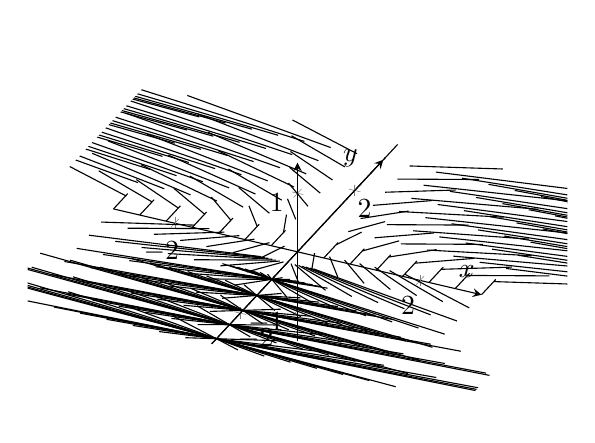
\begin{tikzpicture}
          \begin{axis}[
            axis equal,
            axis lines=middle,
            xmin=-3, xmax=3, ymin=-3, ymax=3,
            xlabel={$x$}, ylabel={$y$},
            samples=15,
            domain=-3:3, y domain=-3:3,
            quiver={
              u={x*y},
              v={0.5},
            },
            every arrow/.append style={-stealth, blue},
          ]
          \addplot3[quiver] {0};
          \end{axis}
        \end{tikzpicture}
    \end{center}
}

\qs{}{
    Given the contour diagram for a function \(f\) shown below, in which dark colors correspond to low values of \(f\) and light colors correspond to high values of \(f\), sketch the gradient vector field \(\vec{F} = \nabla f\).
    \insertpng[0.25]{prob4.png}
}

\sol{
    \begin{center}
        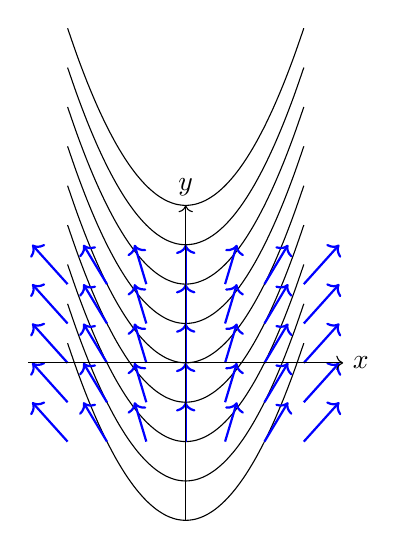
\begin{tikzpicture}
            % Draw the contour lines based on the diagram
            \foreach \i in {-4,-3,...,4} {
                \draw[thin] plot[domain=-1.5:1.5, smooth] (\x,{(\x)^2 - \i/2});
            }
        
            % Add gradient vectors (hypothetical) at sample points
            \foreach \x in {-1.5,-1,-0.5,0,0.5,1,1.5} {
                \foreach \y in {-1,-0.5,0,0.5,1} {
                    % Compute a generic direction for the gradient (upward and away from the center)
                    \draw[->, thick, blue] (\x, \y) -- ++(0.3*\x, 0.5);
                }
            }
        
            % Axes for reference
            \draw[->] (-2,0) -- (2,0) node[right] {$x$};
            \draw[->] (0,-2) -- (0,2) node[above] {$y$};
        \end{tikzpicture}        
    \end{center}
}
\qs{}{
    A thin wire has the shape of the curve \(C\) parameterized by \(x = \cos t\), \(y = \sin t\), \(z = t\), \(0 \leq t \leq 4\pi\), where \(x, y,\) and \(z\) are measured in centimeters. The linear density of the wire is given by \(\rho(x, y, z) = x^2 z\) grams per centimeter. Find the mass of the wire.
}

\sol{
    \[ x = \cos t \quad y = \sin t \quad z = t \]
    \[ 0 \leq t \leq 4\pi \] 
    \[ \rho(x,y,x) = x^{2}z \frac{\text{grams}}{\text{cm}} \] \
    \[ \text{Mass: } = \int\limits_{C} \rho(x,y,z) ds \] 
    \[ \frac{dx}{dt} = - \sin t \quad \frac{dy}{dt} = \cos t \quad \frac{dz}{dt} = 1 \] 
    \[ ds = \sqrt{\left(\frac{dx}{dt}\right)^{2} + \left(\frac{dy}{dt}\right)^{2} + \left(\frac{dz}{dt}\right)^{2} } \, dt \] 
    \[ ds = \sqrt{\left(-\sin(t)\right)^{2} + \left(\cos (t)\right)^{2} + \left(1\right)^{2} } \, dt \]  
    \[ ds = \sqrt{1 + 1} \, dt = \sqrt{2} \, dt \] 
    \[ \rho(x,y,z) = x^{2}z \Rightarrow \cos^{2}t \cdot t \Rightarrow t \cos^{2} t \]
    \[ \text{Mass: } \int_{0}^{4\pi} \rho(t) ds = \int_{0}^{4\pi} t \cos^{2} t \sqrt{2} \, dt \]
    \[ \sqrt{2} \int_{0}^{4} t \cos ^{2} t dt \quad \cos^{2}t = \frac{1 + \cos 2t}{2} \] 
    \[ \sqrt{2} \int_{0}^{4\pi} t \left(\frac{1 + \cos 2t}{2}\right) \, dt \Rightarrow \frac{\sqrt{2}}{2} \int_{0}^{4\pi} t (1 + \cos 2t )\, dt \]
    \[ \frac{\sqrt{2}}{2} \int_{0}^{4\pi} t \, dt + \frac{\sqrt{2}}{2} \int_{0}^{4\pi} t \cos 2t \, dt \] 
    \[ \int_{0}^{4\pi} t \, dt = \left. \frac{t^{2}}{2}\right|_{0}^{4\pi} \Rightarrow \frac{\sqrt{2}}{2} \frac{16 \pi^{2}}{2} - \frac{\sqrt{2}}{2} \frac{0}{2} = 4\sqrt{2}\pi^{2} \] 
    \[ u = t \quad du = dt \]
    \[ v = \frac{1}{2} \sin 2t \quad dv = \cos 2t \]
    \[ \int t \cos 2t \, dt = t \cdot \frac{1}{2} \sin 2t - \int \frac{1}{2} \sin 2t dt = \frac{1}{2} t \sin 2t + \frac{1}{4} \cos 2t + k \]
    \[ \left[ \frac{1}{2} t \sin 2t + \frac{1}{4} \cos 2t \right]_{0}^{4 \pi} = \left( \frac{1}{2} \cdot 4 \pi \cdot 0 + \frac{1}{4} \cdot 1 \right) - \left(0 + \frac{1}{4} \cdot 1\right) = 0 \]
    \[ 4 \sqrt{2} \pi^{2} + 0 = 4 \sqrt{2}\pi^{2} \]       
}

\qs{}{
    Let \(\vec{F}\) be the vector field shown below, and let \(C\) be the unit circle, oriented clockwise. Is the vector line integral
    \[
    \int_C \vec{F} \cdot d\vec{r}
    \]
    positive, negative, or zero? Explain your reasoning.
    \insertpng[0.25]{prob6.png}
}

\sol{ 
    \\ 
    In the first quadrant (top right), the vectors point in the counterclockwise direction. In the second quadrant (top left), the vectors still circulate in a way consistent with a counterclockwise motion.
    In the third and fourth quadrants, the vectors similarly maintain this pattern, suggesting the field is rotating counterclockwise overall. \\
    Since the problem states the circle C is clockwise oriented, the direction of the field is opposite to the direction of the curve's traversal. \\
    The line integral $\int_{C} \vec{F} \, d\vec{r} $ measures the component of the vector field $\vec{F}$
    that aligns with the direction of traversal around the curve C. Here, the vector field rotates counterclockwise, but the traversal of CC is clockwise.
    Since the field vectors mostly oppose the direction of movement along the curve, the dot product $ \vec{F} \cdot \, d \vec{r} $ will tend to be negative along the path.
}

\newpage 

\qs{}{
    Evaluate the line integral 
    \[
    \int_C \sin x \, dx + \cos y \, dy
    \]
    where \(C\) consists of the top half of the circle \(x^2 + y^2 = 1\) from \((1, 0)\) to \((-1, 0)\) and the line segment from \((-1, 0)\) to \((-2, 3)\). (Remember that when you see an integral that looks like 
    \[
    \int_C P(x, y) \, dx + \int_C Q(x, y) \, dy
    \]
    it is a shorthand notation for 
    \[
    \int_C \vec{F}(\vec{r}(t)) \cdot d\vec{r}
    \]
    where \(\vec{F}(x, y) = \langle P(x, y), Q(x, y) \rangle\). The analogous thing is true in three dimensions.)
}

\sol{
    \[
    x^{2} + y^{2} = 1 \quad x = \cos t \quad y = \sin t \quad t \in [0, \pi]
    \]

    \[
    x(t) = (1 - t)(-1) + t(-2) \quad y(t) = (1 - t)(0) + t(3) \quad t \in [0,1]
    \]

    \[
    \vec{F}(x, y) = \langle \sin x, \cos y \rangle
    \]

    \[
    \int\limits_{C} \sin x \, dx + \cos y \, dy
    \]

    \[ 
    x(t) = \cos t, \quad y(t) = \sin t, \quad t \in [0, \pi]
    \]

    \[
    \frac{dx}{dt} = -\sin t, \quad \frac{dy}{dt} = \cos t
    \]

    \[
    \int\limits_{C_1} \sin x \, dx + \cos y \, dy = \int_{0}^{\pi} \left[ \sin(\cos t)(- \sin t) + \cos(\sin t) \cos t \right] dt
    \]

    \[
    \int_{0}^{\pi} \sin(\cos t)(- \sin t) \, dt + \int_{0}^{\pi} \cos(\sin t) \cos t \, dt
    \]

    \[
    f(x, y) = -\cos x + \sin y
    \]

    At \((1, 0)\):
    \[
    f(1, 0) = -\cos(1) + \sin(0) = -\cos(1)
    \]

    At \((-1, 0)\):
    \[
    f(-1, 0) = -\cos(1)
    \]

    \[
    \int\limits_{C_1} \sin x \, dx + \cos y \, dy = f(-1, 0) - f(1, 0) = 0
    \]

    \[
    x(t) = -1 - t, \quad y(t) = 3t, \quad t \in [0, 1]
    \]

    \[
    dx = -1 \, dt, \quad dy = 3 \, dt
    \]

    \[
    \int\limits_{C_2} \sin x \, dx + \cos y \, dy = \int_{0}^{1} \left[ \sin(-1 - t)(-1) + \cos(3t)(3) \right] dt
    \]


    Using \(\sin(-1 - t) = -\sin(1 + t)\), the integral becomes:
    \[
    \int_{0}^{1} \sin(1 + t) \, dt + 3 \int_{0}^{1} \cos(3t) \, dt
    \]

    \[
    \int_{0}^{1} \sin(1 + t) \, dt = -\cos(1 + t) \Big|_0^1 = -\cos(2) + \cos(1)
    \]

    \[
    3 \int_{0}^{1} \cos(3t) \, dt = 3 \left( \frac{1}{3} \sin(3t) \Big|_0^1 \right) = \sin(3)
    \]

    \[
    \int\limits_{C_2} \sin x \, dx + \cos y \, dy = \cos(1) - \cos(2) + \sin(3)
    \]

    \[
    \int\limits_{C} \sin x \, dx + \cos y \, dy = \int\limits_{C_1} \sin x \, dx + \cos y \, dy + \int\limits_{C_2} \sin x \, dx + \cos y \, dy
    \]

    Since \( \int\limits_{C_1} \sin x \, dx + \cos y \, dy = 0 \), the total integral is:
    \[
    \int\limits_{C} \sin x \, dx + \cos y \, dy = \cos(1) - \cos(2) + \sin(3)
    \]

}

\qs{}{
    Compute the line integral of the vector field 
    \[
    \vec{F}(x, y) = \frac{x}{\sqrt{x^2 + y^2}} \hat{\imath} + \frac{y}{\sqrt{x^2 + y^2}} \hat{\jmath}
    \]
    along the parabola \(x = 1 + y^2\) from \((2, -1)\) to \((2, 1)\).
}

\sol{
    \[ \int\limits_{C} \vec{F} \cdot d\vec{r} = \int_{a}^{b} \left[ F_{1} (x(t),y(t)) \frac{dx}{dt} + F_{2}(x(t), y(t)) \frac{dy}{dt} \right] dt \] 
    \[ y = t \quad t \in [-1,1] \quad x(t) = 1 + t^{2} \]
    \[ r(t) = \langle x(t), y(t) \rangle = \langle 1 + t^{2}, t \rangle \quad t \in [-1,1] \] 
    \[ \frac{dx}{dt} = 2t \quad \frac{dy}{dt} = 2 \] 
    \[ \vec{F}(x,y) \Rightarrow \vec{F}(1 + t^{2}, t) =  \frac{1+t^{2}}{\sqrt{\left(1+t^{2}\right)^{2} + t^{2}}} \hat{\imath} +  \frac{t}{\sqrt{\left(1+t^{2}\right)^{2} + t^{2}}} \hat{\jmath} \]
    \[ \left[ \frac{1+t^{2}}{\sqrt{\left(1+t^{2}\right)^{2} + t^{2}}} \times 2t \right] + \left[ \frac{t}{\sqrt{\left(1+t^{2}\right)^{2} + t^{2}}} \times 1 \right] \]
    \[ \int_{a}^{b} \left[ \frac{3t+2t^{3}}{\sqrt{\left(1+t^{2}\right)^{2} + t^{2}}}\right] dt \]
    \[ \int_{a}^{b} \frac{3t+2t^{3}}{\sqrt{1+3t^{2}+t^{4}}} dt \]
    \[ d\vec{r} = (2t \hat{\imath}, 2 \hat{\jmath})\] 
    \[ \vec{F} \cdot d\vec{r} = \frac{3t+2t^{3}}{\sqrt{1+3t^{2}+t^{4}}} \]
    \[ d\frac{d}{dt} \sqrt{1 + 3t^{2} + t^{4}} = \frac{3t + t^{2}}{\sqrt{t^{4} + 3t^{2} + 1}} \] 
    \[ \vec{F} \cdot d\vec{r} = d\left( \sqrt{t^{4} + 3t^{2} + 1} \right)\] 
    \[ \int_{a}^{b} \vec{F} d\vec{r} = \left[ t^{4} + 3t^{2} + 1 \right]_{-1}^{1} = \sqrt{1^{4} + 3(1)^{2} + 1 } - \sqrt{1 + 3(-1)^{2} + (-1)^{4}} = 0 \] 
}

\qs{}{
    Evaluate the line integral of the vector field
    \[
    \vec{F}(x, y, z) = (x + y) \hat{\imath} + (y - z) \hat{\jmath} + z^2 \hat{k}
    \]
    along the path parameterized by 
    \[
    \vec{r}(t) = t^2 \hat{\imath} + t^3 \hat{\jmath} + t^2 \hat{k}, \quad 0 \leq t \leq 1.
    \]
}
\sol{
    \[ \vec{F}(x,y,x) = (x + y) \hat{\imath} + (y - z) \hat{\jmath} + z^2 \hat{k} \] 
    \[ \vec{r}(t) = t^2 \hat{\imath} + t^3 \hat{\jmath} + t^2 \hat{k}, \quad 0 \leq t \leq 1 \]
    \[ \frac{d\vec{r}}{dt} = 2t \, \hat{\imath} + 3t^{2} \hat{\jmath} + 2t \, \hat{k} \]
    \[ \vec{F}(t) = \left[ t^{2} + t^{3} \right] \, \hat{\imath} + \left[ t^{3} - t^{2} \right] \, \hat{\jmath} + \left[ t^{4} \right] \, \hat{k} \]
    \[ \vec{F} \cdot \frac{dr}{dt} = \left[ \left(t^{2} + t^{3} \right)(2t) \right] + \left[ \left(t^{2} - t^{3} \right)\left(3t^{2}\right) \right] + \left[ \left(t^{4}\right)(2t)\right]\]   
    \[ \vec{F} \frac{d\vec{r}}{dt} = 2t^{3} - t^{4} + 5t^{5} \]
    \[ \int_{0}^{1} \left[ 2t^{3} - t^{4} + 5t^{5} \right] dt = \left[ \frac{1}{2}t^- \frac{1}{5}t^{5} + \frac{5t^{6}}{6} \right]_{0}^{1} \]\
    \[ \left( \frac{1}{2} - \frac{1}{5} + \frac{5}{6} \right) - 0 = \frac{17}{15} \]   
}

\newpage 

\qs{}{
    For each of the following vector fields \(\vec{F}\) and curves \(C\), find a function \(f\) such that \(\vec{F} = \nabla f\) and use this function to evaluate 
    \[
    \int_C \vec{F} \cdot d\vec{r}
    \]
    along the given directed curve \(C\).
    \begin{enumerate}
        \item \(\vec{F}(x, y) = \langle x^2, y^2 \rangle\),  
        \(C\) is the arc of the parabola \(y = 2x^2\) from \((-1, 2)\) to \((2, 8)\).

        \item \(\vec{F}(x, y, z) = \langle e^y, xe^y, (z + 1)e^z \rangle\),  
        \(C : \vec{r}(t) = \langle t, t^2, t^3 \rangle\), \(0 \leq t \leq 1\).
    \end{enumerate}
}

\sol{
    \[ F = \nabla f \]
    \[ \int\limits_{C} F \cdot d\vec{r} = f(\text{end point}) - f(\text{start point}) \] 
    Problem 1 
    \[ \frac{\partial f}{\partial x} = x^{2} \quad \frac{\partial f}{\partial y} = y^{2} \]
    \[ f(x,y) = \int x^{2} \, dx = \frac{1}{3}x^{2} + g(y) \]
    \[ \frac{\partial g}{\partial y} = g'(y) = y^{2} \]
    \[ g(y) = \int_ y^{2} \, dy = \frac{1}{3}y^{3} \]
    \[ f(x,y) = \frac{1}{3}x^{3} + \frac{1}{3}y^{3} \]
    \[ \int F \, d\vec{r} = f(2,8) - f(-1,2) = 171 \] 
    Problem 2
    \[ \vec{F}(x,y,z) = \langle e^{y}, xe^{y}, (z + 1)e^{z} \rangle \quad \vec{r}(t) = \left(t,t^{2}, t^{3}\right) \]    
    \[ \frac{\partial F}{x} = e^{x} \quad \frac{\partial F}{\partial y} = xe^{y} \quad \frac{\partial F}{\partial z} = (z+1)e^{z} \] 
    \[ f(x,y,z) = \int e^{y} \, dx = xe^{y} + \rho(y,z) \]
    \[ \frac{\partial f}{\partial y} = xe^{y} + \frac{\partial \rho}{\partial y} \quad xe^{y} + \frac{\partial \rho}{\partial y} \quad \frac{\partial \rho}{\partial y} = 0 \]
    \[ \rho(x,y,z) = \phi(z) \]
    \[ \frac{\partial f}{\partial z} = (z+1)e^{z} \]
    \[ \rho(z) = \int (z+1)e^{z} \, dz \]
    \[ u = z + 1 \quad du = 1 \, dz \] 
    \[ v = e^{z} \, dv = e^{z} \, dz \] 
    \[ \int (z+1)e^{z} \, dz = (z+1) e^{z} - \int e^{z} \, dz \] 
    \[ (z+1)e^{z} - e^{z} \Rightarrow ze^{z} + e^{z} - e^{z} = ze^{z} \]
    \[ f(x,y,z) = xe^{y} + ze^{z} \]
    \[ f(1,1,1) = (1)e^{1} + (1)e^{1} = ze \] 
    \[ f(0,0,0) = (0)e^{0} + + (0)e^{0} = 0 \]
    \[ \int\limits_{C} \vec{F} \cdot d\vec{r} = f(1,1,1) - f(0,0,0) = 2e \]          
}

\qs{}{
    Clairaut's Theorem implies that if the vector field \(\vec{F} = P \hat{\imath} + Q \hat{\jmath} + R \hat{k}\) is conservative and \(P, Q,\) and \(R\) have continuous first-order partial derivatives, then
    \[
    \frac{\partial P}{\partial y} = \frac{\partial Q}{\partial x}, \quad 
    \frac{\partial P}{\partial z} = \frac{\partial R}{\partial x}, \quad 
    \frac{\partial Q}{\partial z} = \frac{\partial R}{\partial y}.
    \]
    \begin{enumerate}
        \item Use the statement above to show that the vector line integral
        \[
        \int_C x \, dx + 2x \, dy + xz \, dz
        \]
        is not independent of path.

        \item Find two directed curves \(C_1\) and \(C_2\) that start at the same point and end at the same point, such that
        \[
        \int_{C_1} x \, dx + 2x \, dy + xz \, dz \neq \int_{C_2} x \, dx + 2x \, dy + xz \, dz.
        \]
    \end{enumerate}
}

\sol{ 
    \\
    a) 
    \[
    \frac{\partial P}{\partial y} = \frac{\partial Q}{\partial x}, \quad 
    \frac{\partial P}{\partial z} = \frac{\partial R}{\partial x}, \quad 
    \frac{\partial Q}{\partial z} = \frac{\partial R}{\partial y}.
    \]

    \[
    P = x, \quad Q = 2x, \quad R = xz.
    \]

    \[
    \frac{\partial P}{\partial y} = \frac{\partial x}{\partial y} = 0, \quad 
    \frac{\partial Q}{\partial x} = \frac{\partial 2x}{\partial x} = 2.
    \]

    \[
    \frac{\partial P}{\partial z} = \frac{\partial x}{\partial z} = 0, \quad 
    \frac{\partial R}{\partial x} = \frac{\partial (xz)}{\partial x} = z.
    \]

    \[
    \frac{\partial Q}{\partial z} = \frac{\partial 2x}{\partial z} = 0, \quad 
    \frac{\partial R}{\partial y} = \frac{\partial (xz)}{\partial y} = 0.
    \]

    The first inequality does not hold true nor does teh second but third does. This means that it is not conservative \\

    b) 
    \[
    \int_C x \, dx + 2x \, dy + xz \, dz
    \]

    \[
    A = (0, 0, 0), \quad B = (1, 0, 0)
    \]

    \[
    x = t, \quad y = 0, \quad z = 0, \quad t \in [0, 1]
    \]

    \[
    dx = dt, \quad dy = 0, \quad dz = 0
    \]

    \[
    \int_{C_1} x \, dx + 2x \, dy + xz \, dz = \int_{0}^{1} t \, dt = \left[ \frac{1}{2} t^2 \right]_0^1 = \frac{1}{2}
    \]

    \[
    C_2: \quad C_{2a}, \quad C_{2b}, \quad C_{2c}
    \]

    \[
    C_{2a}: \quad (0, 0, 0) \to (0, 1, 0)
    \]

    \[
    x = 0, \quad y = t, \quad z = 0, \quad t \in [0, 1]
    \]

    \[
    dx = 0, \quad dy = dt, \quad dz = 0
    \]

    \[
    \int_{C_{2a}} x \, dx + 2x \, dy + xz \, dz = \int_{0}^{1} 0 \, dt = 0
    \]

    \[
    C_{2b}: \quad (0, 1, 0) \to (1, 1, 0)
    \]

    \[
    x = t, \quad y = 1, \quad z = 0, \quad t \in [0, 1]
    \]

    \[
    dx = dt, \quad dy = 0, \quad dz = 0
    \]

    \[
    \int_{C_{2b}} x \, dx + 2x \, dy + xz \, dz = \int_{0}^{1} t \, dt = \left[ \frac{1}{2} t^2 \right]_0^1 = \frac{1}{2}
    \]

    \[
    C_{2c}: \quad (1, 1, 0) \to (1, 0, 0)
    \]

    \[
    x = 1, \quad y = t, \quad z = 0, \quad t \in [1, 0]
    \]

    \[
    dx = 0, \quad dy = dt, \quad dz = 0
    \]

    \[
    \int_{C_{2c}} x \, dx + 2x \, dy + xz \, dz = 2 \int_{1}^{0} dt = 2 (0 - 1) = -2
    \]

    \[
    \int_{C_2} = \int_{C_{2a}} + \int_{C_{2b}} + \int_{C_{2c}} = 0 + \frac{1}{2} + (-2) = -\frac{3}{2}
    \]

    \[
    \int_{C_1} x \, dx + 2x \, dy + xz \, dz = \frac{1}{2}
    \]

    \[
    \int_{C_2} x \, dx + 2x \, dy + xz \, dz = -\frac{3}{2}
    \]

    \[
    \frac{1}{2} \neq -\frac{3}{2}
    \]

    \[
    \int_{C_1} x \, dx + 2x \, dy + xz \, dz \ne \int_{C_2} x \, dx + 2x \, dy + xz \, dz
    \]

}

\newpage 

\qs{}{
    The force exerted by an electric charge at the origin on a charged particle at a point \((x, y, z)\) with position vector \(\vec{r} = \langle x, y, z \rangle\) is 
    \[
    \vec{F}(\vec{r}) = K \frac{\vec{r}}{|\vec{r}|^3},
    \]
    where \(K\) is a constant. Find the work done on the particle as it moves along the straight line from \((0, 3, 0)\) to \((1, 3, 2)\) in two ways:
    \begin{enumerate}
        \item Parameterize the line segment, and compute 
        \[
        \int_a^b \vec{F}(\vec{r}(t)) \cdot \vec{r}'(t) \, dt
        \]
        directly.
        
        \item Although \(\vec{F}\) is not defined at the origin, it turns out that \(\vec{F}\) is conservative on its domain. Find a potential function \(f\), and use the Fundamental Theorem of Line Integrals to compute the work done on the particle.
    \end{enumerate}
}

\sol{
    \\
    a) 
    \[
    \vec{r}(t) = (t, 3, 2t), \quad t \in [0, 1]
    \]
    \[
    \vec{r}'(t) = \langle 1, 0, 2 \rangle
    \]
    \[
    |\vec{r}(t)| = \sqrt{5t^2 + 9}
    \]
    \[
    \vec{F}(\vec{r}(t)) = K \frac{\langle t, 3, 2t \rangle}{(5t^2 + 9)^{3/2}}
    \]
    \[
    \vec{F}(\vec{r}(t)) \cdot \vec{r}'(t) = K \frac{5t}{(5t^2 + 9)^{3/2}}
    \]
    \[
    W = \int_0^1 K \frac{5t}{(5t^2 + 9)^{3/2}} \, dt
    \]
    Substitution: \( u = 5t^2 + 9 \), \( du = 10t \, dt \)
    \[
    W = K \int_9^{14} \frac{du}{2u^{3/2}}
    \]
    \[
    W = \frac{K}{2} \int_9^{14} u^{-3/2} \, du
    \]
    \[
    W = -K \left[ u^{-1/2} \right]_9^{14} = K \left( \frac{1}{3} - \frac{1}{\sqrt{14}} \right)
    \]

    b) 
    \[
    f(\vec{r}) = -\frac{K}{|\vec{r}|}
    \]
    \[
    W = f(\vec{r}_B) - f(\vec{r}_A)
    \]
    \[
    |\vec{r}_A| = 3, \quad |\vec{r}_B| = \sqrt{14}
    \]
    \[
    W = K \left( \frac{1}{3} - \frac{1}{\sqrt{14}} \right)
    \]
}

\end{document}